% -*- TeX-engine: luatex -*-
\documentclass[presentation,aspectratio=43,10pt]{beamer}
\usepackage{pgfplots}
\pgfplotsset{compat=1.15}
\usepackage{template}
\renewcommand{\authorname}{Lawrence Mitchell\inst{*}}
\renewcommand{\authoremail}{\inst{*}\texttt{lawrence.mitchell@durham.ac.uk}}

\renewcommand{\sessionnumber}{4}
\renewcommand{\sessiontitle}{Performance measurements}
\usepackage{tikz}
\usetikzlibrary{matrix,fit,positioning,calc}
\usepackage{pgfplotstable}
\usetikzlibrary{pgfplots.groupplots}
\date{}

\begin{document}
\begin{frame}
  \maketitle
\end{frame}

\begin{frame}
  \frametitle{Roofline dense matrix-vector product}
  \begin{center}
    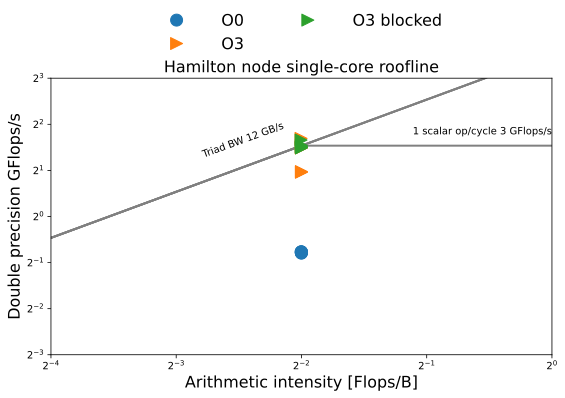
\includegraphics[width=0.9\textwidth]{figures/roofline-dmvm}
  \end{center}
\end{frame}
\begin{frame}
  \frametitle{How and what to measure}
  \begin{itemize}
  \item Roofline gives us a high-level overview of what to try next.
  \item How to drill down and get more information about what is
    causing the bottleneck?
  \item How to confirm the hypothesis formed through the roofline
    analysis?
  \item[$\Rightarrow$] \emph{Measure} things about the code.
  \end{itemize}
\end{frame}

\begin{frame}
  \frametitle{Performance measurements}
  \begin{itemize}
  \item Modern hardware comes with some special purpose
    \emph{registers} that you can prod to measure low level
    performance events.
  \item Can use this to characterise performance of a piece of code
  \end{itemize}
  \begin{block}{Caveats}
    \begin{itemize}
    \item Measurements can only tell you about the algorithm you're
      using
    \item e.g.~Counts the data you moved, not the data you could have
      moved.
    \item Do not tell you about potential better algorithms
    \item Need to work hand in hand with models.
    \end{itemize}
  \end{block}
\end{frame}

\begin{frame}
  \frametitle{What kind of things can we measure?}
  \begin{itemize}
  \item An almost overwhelming number of different things like:
    \begin{itemize}
    \item Number of floating point instructions of different type
      (scalar, sse, avx)
    \item Cache miss/hit counts at various levels
    \item Branch prediction success rate
    \item \dots
    \end{itemize}
  \item[$\Rightarrow$] Best used to confirm hypothesis from some model
  \end{itemize}
\end{frame}

\begin{frame}
  \frametitle{Abstract metrics}
  \begin{itemize}
  \item Can read low-level hardware counters directly (e.g.~how many
    floating point instructions were executed?)
  \item More useful to group into abstract metrices
  \item[$\Rightarrow$] easier to compare across hardware, easier to
    interpret.
  \item For example, measure ``Instructions per cycle'' rather than
    instructions.
  \end{itemize}
\end{frame}

\begin{frame}
  \frametitle{How do we measure them?}
  \begin{itemize}
  \item Use \texttt{likwid-perfctr} (installed on Hamilton via the
    \texttt{likwid} module).
  \item Offers a reasonably friendly command-line interface.
  \item Provides access both to counters directly, and many useful
    predefined ``groups''.
  \end{itemize}
\end{frame}

\begin{frame}[fragile]
  \frametitle{Example: STREAM}
  \begin{itemize}
  \item Will use \texttt{likwid-perfctr} to measure memory references
    in different implementations of the same loop.
  \end{itemize}
  \begin{columns}[t]
    \begin{column}{0.25\textwidth}
      \begin{block}{Scalar}
\begin{minted}[fontsize=\tiny]{asm}
for i from 0 to n:
  load a[i:i+1] reg1
  load b[i:i+1] reg2
  load c[i:i+1] reg4
  mul reg1 reg2 reg3
  add reg4 reg3 reg4
  store reg4 c[i:i+1]
\end{minted}
      \end{block}
    \end{column}
    \begin{column}{0.25\textwidth}
      \begin{block}{SSE}
\begin{minted}[fontsize=\tiny]{asm}
for i from 0 to n by 2:
  vload a[i:i+2] vreg1
  vload b[i:i+2] vreg2
  vload c[i:i+2] vreg4
  vmul vreg1 vreg2 vreg3
  vadd reg4 reg3 reg4
  vstore reg4 c[i:i+2]
\end{minted}
      \end{block}
    \end{column}
    \begin{column}{0.25\textwidth}
      \begin{block}{AVX}
\begin{minted}[fontsize=\tiny]{asm}
for i from 0 to n by 4:
  vload a[i:i+4] vreg1
  vload b[i:i+4] vreg2
  vload c[i:i+4] vreg4
  vmul vreg1 vreg2 vreg3
  vadd reg4 reg3 reg4
  vstore reg4 c[i:i+4]
\end{minted}
      \end{block}
    \end{column}
    \begin{column}{0.25\textwidth}
      \begin{block}{AVX2}
\begin{minted}[fontsize=\tiny]{asm}
for i from 0 to n by 4:
  vload a[i:i+4] vreg1
  vload b[i:i+4] vreg2
  vload c[i:i+4] vreg3
  vfma vreg1 vreg2 vreg3
  vstore reg3 c[i:i+4]
\end{minted}
      \end{block}
    \end{column}
  \end{columns}
\end{frame}

\begin{frame}
  \frametitle{Measurement}
  \begin{challenge}{Model}
    For each loop choice, if we choose $n = 10^6$, how many load
    and store instructions do we expect to measure?
  \end{challenge}
  \pause
  \begin{answer}{Answer}
    Each loop iteration has 3 loads and 1 store.

    Vector width $v$ and $n$ iterations we need $\frac{3n}{v}$ loads
    and $\frac{n}{v}$ stores.

    $\Rightarrow$ let's attempt to verify this with measurements.
  \end{answer}
\end{frame}

\begin{frame}
  \frametitle{Exercise}
  \begin{itemize}
  \item Goal is to convince ourselves that measurement works!
  \item[$\Rightarrow$] Exercise 5 from the usual place.
  \end{itemize}

\end{frame}

\begin{frame}
  \frametitle{Larger code}
  \begin{challenge}{Problem}
    What if you don't know which part of the code takes all the time?
  \end{challenge}
  \begin{answer}{Answer}
    Use \emph{profiling} to determine hotspots (regions of code where
    all the time is spent).

    $\Rightarrow$ allows us to focus in on important parts.
  \end{answer}
\end{frame}

\begin{frame}
  \frametitle{Profiling: types}
  \begin{itemize}
  \item Goal is to gather information about what a code is doing
    \begin{itemize}
    \item \emph{Sampling}
    \item or \emph{code instrumentation}
    \end{itemize}
  \end{itemize}
  \begin{columns}
    \begin{column}{0.45\textwidth}
      \begin{exampleblock}{Sampling}
        \begin{itemize}
        \item Works with unmodified executables
        \item Only a statistical model of code execution
        \item[$\Rightarrow$] not very detailed for volatile metrics
        \item[$\Rightarrow$] needs long-running application
        \end{itemize}
      \end{exampleblock}
    \end{column}
    \begin{column}{0.45\textwidth}
      \begin{exampleblock}{Instrumentation}
        \begin{itemize}
        \item Requires source code annotations to capture
          ``interesting'' information
        \item Much more details and focused
        \item[$\Rightarrow$] Preprocessing of source required
        \item[$\Rightarrow$] Can have large \emph{overheads} for small functions.
        \end{itemize}
      \end{exampleblock}
    \end{column}
  \end{columns}
\end{frame}

\begin{frame}
  \frametitle{Sampling}
  \begin{itemize}
  \item Running program is periodically interrupted to take a measurement.
  \item Records which function we are in.
  \end{itemize}
  \begin{center}
    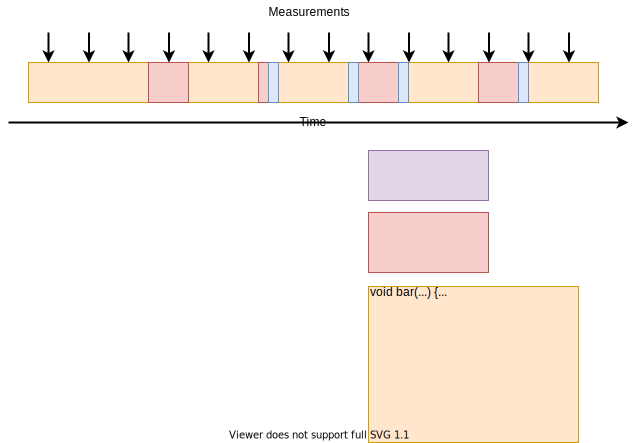
\includegraphics[height=0.6\textheight]{figures/samplingprofile}
  \end{center}
\end{frame}
\begin{frame}
  \frametitle{Tracing}
  \begin{itemize}
  \item Measurement code is inserted to capture all the events we care
    about
  \end{itemize}
  \begin{center}
    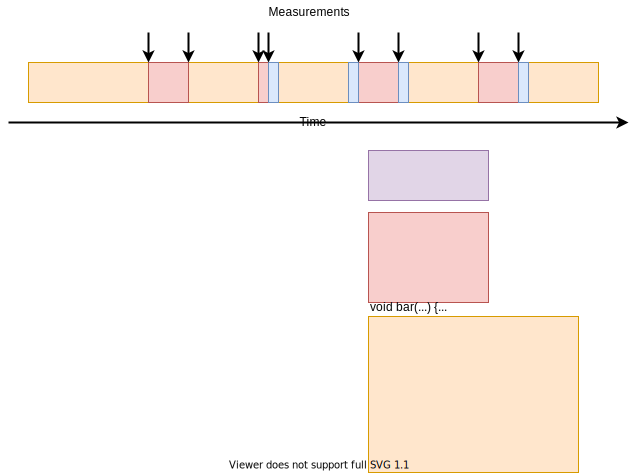
\includegraphics[height=0.7\textheight]{figures/tracingprofile}
  \end{center}
\end{frame}


\begin{frame}
  \frametitle{Sampling profiles with gprof}
  \begin{exampleblock}{Workflow}
    \begin{enumerate}
    \item Compile \emph{and link} code with symbols (add \texttt{-g}) and profile
      information (\texttt{-p}).
    \item Run code $\Rightarrow$ produces file \texttt{gmon.out}
    \item Postprocess data with \texttt{gprof}
    \item Look at results
    \end{enumerate}
  \end{exampleblock}
\end{frame}

\begin{frame}[fragile]
  \frametitle{gprof ``flat profile''}
\begin{minted}[fontsize=\scriptsize]{sh}
Flat profile:

Each sample counts as 0.01 seconds.
  %   cumulative   self              self     total
 time   seconds   seconds    calls   s/call   s/call  name
 76.14      5.71     5.71      102     0.06     0.06  ForceLJ::compute(Atom&, Neighbor&, Comm&, int)
 17.07      6.99     1.28        6     0.21     0.22  Neighbor::build(Atom&)
  2.80      7.20     0.21        3     0.07     0.07  void ForceLJ::compute_halfneigh<1, 1>(Atom&, Neighbor&, int)
  1.47      7.31     0.11        1     0.11     7.05  Integrate::run(Atom&, Force*, Neighbor&, Comm&, Thermo&, Timer&)
  0.93      7.38     0.07                             __intel_avx_rep_memcpy
  0.40      7.41     0.03       11     0.00     0.00  Neighbor::binatoms(Atom&, int)
  0.40      7.44     0.03        6     0.01     0.01  Comm::borders(Atom&)
  0.40      7.47     0.03        1     0.03     0.04  create_atoms(Atom&, int, int, int, double)
  0.13      7.48     0.01   285585     0.00     0.00  Atom::unpack_border(int, double*)
\end{minted}
\end{frame}
\begin{frame}
  \frametitle{gprof ``flat profile''}
  \begin{itemize}
  \item Code is instrumented (instructions inserted so we know which
    function we're in), triggering of measurement is sampling based
    (not every call).
  \item GProf provides profile with some tracing information
  \item Gives both \emph{inclusive} and \emph{exclusive} timings.
  \end{itemize}
  \begin{columns}
    \begin{column}{0.45\textwidth}
      \begin{itemize}
      \item Blue box shows ``inclusive'' time for \texttt{main}
      \item \texttt{foo} and \texttt{bar} calls (orange) excluded for
        ``exclusive'' time.
      \item[$\Rightarrow$] exclusive time measures execution in
        function that is not attributable to some other function.
      \end{itemize}
    \end{column}
    \begin{column}{0.45\textwidth}
      \begin{center}
        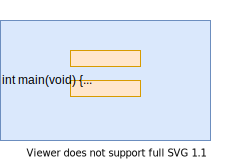
\includegraphics[width=\textwidth]{figures/inclusiveexclusive}
      \end{center}
    \end{column}
  \end{columns}
\end{frame}

\begin{frame}
  \frametitle{Continued workflow}
  \begin{itemize}
  \item After we have identified the hotspot that takes all the time,
    we'd like to determine if it is optimised
  \item[$\Rightarrow$] need more detailed insights.
  \end{itemize}
  \begin{enumerate}
  \item Find relevant bit of code
  \item Determine algorithm
  \item Add instrumentation markers (see exercise)
  \item Profile with more detail/use performance models.
  \item[$\Rightarrow$] guidance for appropriate optimisation.
  \end{enumerate}
\end{frame}
\begin{frame}
  \frametitle{Exercise: finding the hotspot}
  \begin{itemize}
  \item So far, we've looked at very simple code. Now, your task will
    be to find the hotspot and do some exploration in a larger one.
  \item[$\Rightarrow$] Exercise 6 from the usual place.
  \end{itemize}
\end{frame}
\end{document}
